\documentclass[a4paper,9pt]{scrartcl}
\usepackage{amssymb, amsmath} % needed for math
\usepackage[margin=2.5cm]{geometry} %layout
\usepackage[hyperfootnotes=false, pdfborder={0 0 0}, colorlinks=false]{hyperref}
\usepackage{color}
\usepackage{framed}
\usepackage{enumerate}
\usepackage{csquotes} 
\usepackage{listings}
\usepackage{color}
\usepackage{graphicx}


\definecolor{dkgreen}{rgb}{0,0.6,0}
\definecolor{gray}{rgb}{0.5,0.5,0.5}
\definecolor{mauve}{rgb}{0.58,0,0.82}

\lstset{frame=tb,
  language=Python,
  aboveskip=3mm,
  belowskip=3mm,
  showstringspaces=false,
  columns=flexible,
  basicstyle={\small\ttfamily},
  numbers=none,
  numberstyle=\tiny\color{gray},
  keywordstyle=\color{blue},
  commentstyle=\color{dkgreen},
  stringstyle=\color{mauve},
  breaklines=true,
  breakatwhitespace=true,
  tabsize=3
}

\setlength{\parskip}{0.4em}
\setlength{\parindent}{3em} 

\makeatletter
\renewcommand{\subsection}{\@startsection{subsection}{2}{0mm}
  {0.25\baselineskip} 
  {0.25\baselineskip} 
  {\normalfont\normalsize\bfseries}}
\makeatother

\makeatletter
\renewcommand{\section}{\@startsection{section}{1}{0mm}
  {1.5\baselineskip}
  {1\baselineskip} 
  {\normalfont\Large\bfseries}}
\makeatother






\newcommand\titletext{"Self-Favoring Bias in LLMs for Informal-Formal Style Transfer and Potential Propagation into Trained Models"\\ 
\textit{Advanced Natural Language Processing} \\[0.5em] 
\textit{MSc, Artificial Intelligence, 2025}}
\title{\titletext}
\author{Michael Rice}
\usepackage{microtype}

\begin{document}

\maketitle
\section{Project Introduction (200 Words)}

This study investigates whether large language models (LLMs) exhibit a preference for their own generated 
outputs over those produced by other LLMs and whether this bias propagates through models trained on such 
data. To explore this question, the task of informal-to-formal style transfer was selected as a case study.
Three novel, task-specific datasets were constructed to facilitate this analysis. 
These datasets were derived from social media comments, which served as examples of informal text, and 
subsequently transformed into formal text using three distinct LLMs. Once generated, these datasets were
employed to train two model architectures: a foundational Long Short-Term Memory (LSTM) network, developed 
and trained from scratch, and a fine-tuned Sequence-to-Sequence Transformer model, BART 
\cite{lewisBARTDenoisingSequencetoSequence2019}.

The evaluation of the proposed approach was conducted in two stages. First, the models' performance on the
base style transfer task was assessed using standard quantitative metrics, including BLEU score 
\cite{papineniBleuMethodAutomatic2002}. Second, and of greater significance to this study, the three 
LLMs initially used for dataset creation were subsequently leveraged as evaluation tools to assess the 
quality of the style transfer outputs. This evaluation was performed both on the original dataset and on 
the outputs produced by the trained models.

\begin{figure}[h]
\centering
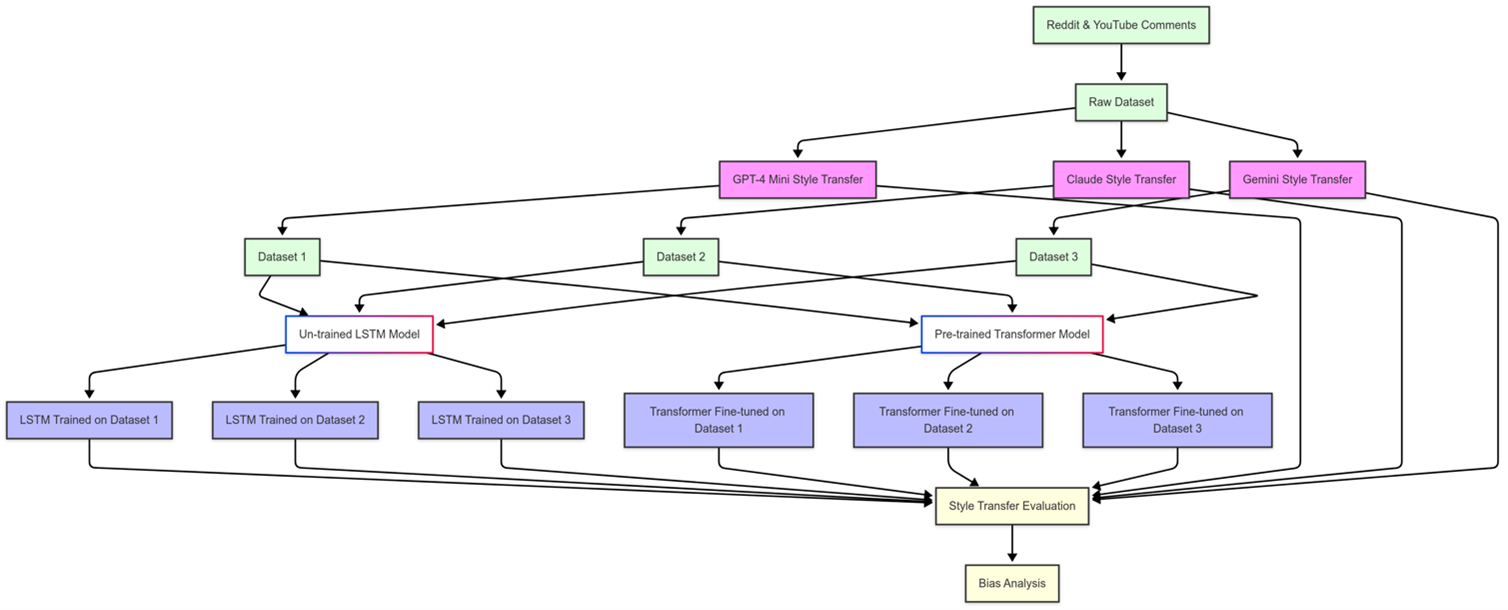
\includegraphics[width=0.8\textwidth]{/home/athen/files/assignments/NLP_Report/NLPProject.png}
\caption{Project Flow Diagram}
\label{fig:style_transfer_example}
\end{figure}


% Finally, a number of sub-experiments were then conducted into the correlation between the 



\section{My Contribution - Dataset Creation (800 Words)}


\subsection{Methodology/Tools (410/400 Words)}

My contribution to this study concerned the generation of the three datasets to be used for
training and evaluation purposes. These datasets each consisted of 50,000 
informal-to-formal sentence pairs. The informal data was gathered through two main methods: scraping 
YouTube comments using YouTube's Data API, as well as filtering and repurposing already gathered Reddit 
comments \cite{zotero-400}. When using the YouTube API, a number of constraints were implemented in an 
attempt to ensure the highest quality data possible. First, only 100 comments were taken from each video,
increasing the number of videos sampled, and thus also increasing the diversity of the dataset. Second, 
potential videos were ordered by view count, as more popular videos were more likely to have at least 100 
comments. Finally, comments from each video were ordered by the number of likes, with the top 100 being 
selected, to further reduce noise in the dataset.


\begin{lstlisting}
#sample video retrieval request
request = youtube.search().list(
        part="id",
        order="viewCount",
        type="video",
        maxResults=50
    )

#sample comment retrieval request
request = youtube.commentThreads().list(
            part="snippet",
            videoId=video_id,
            maxResults=COMMENTS_PER_VIDEO,
            order="relevance",
            textFormat="plainText"
        )
\end{lstlisting}



Due to the ease of access of the Reddit data, this was decided to be the primary source of
informal text, with the final dataset split being 80/20 Reddit/YouTube. To promote the development of a 
well-generalized model, the Reddit data was pre-filtered based on the subreddit of origin before being 
converted into formal text. Finally, before the formal conversion took place, the informal text was cleaned,
as will be detailed in the Challenges section.

\begin{lstlisting}
#subreddit filtering process
wanted_subreddits = [
    'gaming', 'news', 'politics', 'AskReddit', 'teenagers', 'funny',
    'relationship_advice', 'nba', 'AmItheAsshole', 'videos', 'movies',
    'marvelstudios', 'memes', 'soccer', 'todayilearned', 'nfl',
    'trashy', 'unpopularopinion', 'Showerthoughts', 'wallstreetbets']
\end{lstlisting}


The associated formal conversions were generated using three LLMs, each from different providers, OpenAI's 
GPT-4o mini, Meta's Llama Instruct Turbo 70B and Google's Gemini 2.0 Flash. Each LLM was used with a 
temperature of 0.3, to control and compare the creativity of each model. Pandas DataFrames were used as the
tool of choice for dataset storage and manipulation, with the final datasets being saved as CSV files.

Following the conversion of the informal sentences into formal ones, the data was then merged and filtered
to ensure consistency across the three datasets. The reasons this was necessary was due to each API refusing 
or failing to process different input sentences, as well as producing unusual outputs in some cases. This 
filtering involved removing rogue leading characters that appeared, such as \verb|'&gt;'| or speech marks,
matching pairs of sentences between datasets, ensuring sentences did not exceed the max length and removing 
any times the LLMs refused to process a sentence.

\begin{lstlisting}
#ensuring sentence consistency in both the youtube and reddit comments
common_yt = gemini_yt_informal & llama_yt_informal & gpt_yt_informal
common_reddit = gemini_reddit_informal & llama_reddit_informal & gpt_reddit_informal

#refusal to reply removal
final_gemini_reddit = final_gemini_reddit[~final_gemini_reddit['formal'].str.contains('Do not state any reasoning.', na=False)]
reddit_llama = reddit_llama[~reddit_llama['formal'].str.contains('Do not state any reasoning.', na=False)]
final_gpt_reddit = final_gpt_reddit[~final_gpt_reddit['formal'].str.contains('Do not state any reasoning.', na=False)]
\end{lstlisting}

Finally, all three datasets were thoroughly checked to ensure their validity for the task at hand, including
the aforementioned check to ensure the same exact sentences were present in each dataset. 

\begin{lstlisting}
#checking the informal sentences are the same across all datasets
res_final = filtered_gemini_reddit['informal'].equals(filtered_llama_reddit['informal']) and \
            filtered_llama_reddit['informal'].equals(filtered_gpt_reddit['informal'])
\end{lstlisting}



\subsection{Challenges (235/200 Words)}

A number of challenges were faced during this process, with none being more prevalent than dealing with 
each of the LLM API's rate limits, especially in the case of OpenAI's offering. Due to the cost of removing 
such limits, we were limited to using the first paid tier, Tier 1, which limited request to 10000 per day. 
This was a significant bottleneck in project progress as it meant the synthetic pair generation for just 
the OpenAI model took over a week on its own. 

Another challenge encountered during the generation of formal texts was the presence of unsuitable data 
within the informal text set. Prior to the conversion process, the dataset contained texts that were in 
other languages, spanned multiple lines, or were too short. Addressing issues such as multiline comments 
and excessively short comments was relatively straightforward, requiring only a few lines of code from the
function outlined below.

\begin{lstlisting}
#function to remove comments shorter than 5 tokens and to split comments into sentences
def split_and_filter_comments(comments):
    split_comments_list = []
    for comment in comments:
        sentences = nltk.sent_tokenize(comment)
        filtered_sentences = [s for s in sentences if len(s.split()) >= 5]
        filtered_sentences = [s for s in filtered_sentences if len(s.splitlines()) == 1]
        split_comments_list.extend(filtered_sentences)
    return pd.Series(split_comments_list)
  \end{lstlisting}

  
However, the problem of language filtering proved to be more challenging. Due to the absence of a 
suitably effective language detection library — potentially due to difficulty with the 
informal nature of the text — it was determined that the LLMs themselves could be leveraged for this task. 
Specifically, the prompt was augmented to instruct the model to output an 'X' if the input contained 
any non-English terms, thereby enabling the automatic filtering of non-English text during the generation
of the formal portion of the datasets. The resulting pairs could thus be filtered from the output, 
post-generation. 

\begin{lstlisting}
prompt = (
        f"""You are a language model that helps with converting informal text to formal text.
        Please ensure the following sentence is fully formal, grammatically correct, no 
        more than ten tokens longer than the input sequence and only one line. If the input
        comment contains any terms that are not in English, simply return an 'X' as the 
        output. Return only the converted sentence. The informal sentence is: {informal}."""
    )
\end{lstlisting}

git remote add origin https://github.com/monishkajha17/my-first-nft.git
git branch -M main
git push -u origin main


\subsection{Approach Evaluation (100 Words)}

- three, diverse, high-quality datasets created.
- perhaps would alter OpenAI approach should this be tackled again, more automated approach.

The result of this portion of the study was three diverse, high-quality, self-crafted datasets


\subsection{Alternative/Additional Techniques (100 Words)}

When considered potential avenues for future improvements to this process or alternative methods that could 
be utilized to improve the quality of the datasets, the following were identified:


- Increase source diversity.
- Increase base task diversity.
- Increase model diversity.
- Increase dataset size.


\rule{\linewidth}{0.2mm}
\bibliographystyle{plain}
\bibliography{/mnt/c/Users/athen/Desktop/MAI_Sem2/AdvancedNLP/Project/NLP_Report.bib}

\end{document}

